\section{SVM method}

Support-vector machine (SVM) model is supervised machine learning model used for classification. It projects original data point into higher dimension and perform maximal-margin classification in this higher dimension space. 

\todo[inline, color=yellow]{zdroj na svm}

We can use this property and train SVM to classify input tuples of size $k$ to two classes
\begin{enumerate}
    \item \textbf{On line}\\
    This class represents k size ordered tuples with their point laying on the line with same distances between points in tuple. Each two adjacent points in tuple have to be equally distant and  lay on the same straight line.
    
    \item \textbf{Not on line}\\
    This class represents k size tuples which are not \textit{on line}
\end{enumerate}

\begin{figure}[!h]
\centering
\begin{subfigure}{.4\textwidth}
  \centering
  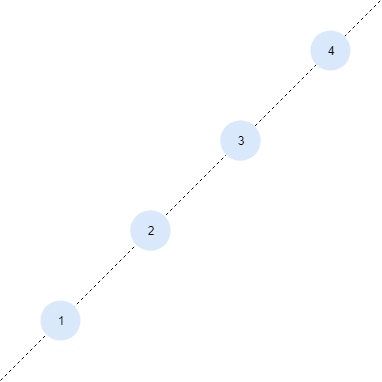
\includegraphics[width=1.0\linewidth]{chapters/images/svm_class1.PNG}
  \caption{On line class example}
  \label{fig:svm_class2}
\end{subfigure}%
\begin{subfigure}{.37\textwidth}
  \centering
  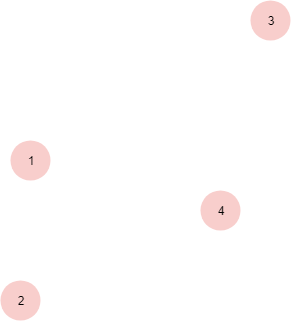
\includegraphics[width=1.0\linewidth]{chapters/images/svm_class2.PNG}
  \caption{Not on line class example }
  \label{fig:svm_class1}
\end{subfigure}
\caption{SVM classification classes}
\label{fig:svm_classes}
\end{figure}

\subsection{Algorithm}

\begin{figure}[!h]
    \centering
    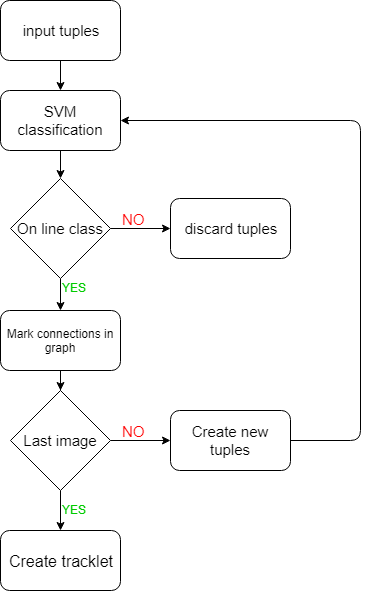
\includegraphics[height=12cm]{chapters/images/SVM_activity_diagram2.PNG}
    \caption{SVM method activity diagram}
    \label{fig:svm_activity_diagram}
\end{figure}

\textbf{Input tuple} consist of $k$ positions $[x, y]$. First position of object in tuple is position of an object from $i$-th image's .tsv file, second from $(i+1)$-th image's file and so on. Last position in tuple is from $(i+k)$-th image's .tsv file. Initially tuples are created by applying Cartesian product between positions of objects from first $k$ images. This process will create $n^k$ tuples if $n$ is number of positions in one image 

Tuple is classified with \textbf{SVM classifier} to one of two classes:
On line class, not on line class. \textbf{Not on line} class tuples are discarded and further proceed only \textbf{on line} class tuples

If result of classifier is \textit{On line}, connections between positions in tuple are marked in graph. 

If tuple last element is not position from last image, \textbf{new tuples are created}. First element is removed from tuple, and at the end one position from next image is appended. New tuple will be created for every position from last image.

After processing all input tuples, we find path from position from first image to some position from last image. If such path exists we consider it as \textbf{tracklet} Positions on the path are positions of moving object.

\begin{figure}[!h]
    \centering
    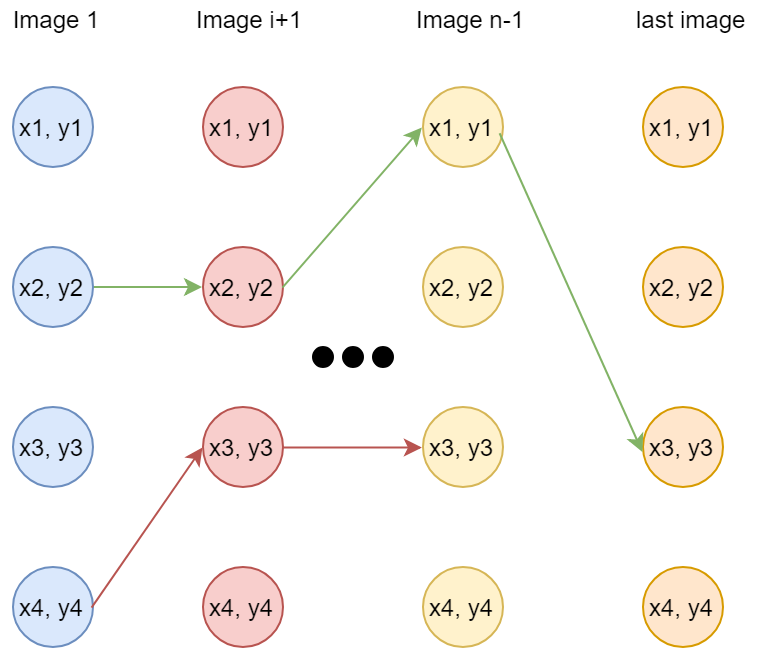
\includegraphics[width=0.8\linewidth]{chapters/images/SVM_graph.PNG}
    \caption{Possible connections in final graph after processing images}
    \label{fig:svm_result_graph}
\end{figure}

In figure \ref{fig:svm_result_graph} there are two possible paths. Green one leads from first image to last image therefore can be declared as tracklet. Nodes in graph are position of moving object in tracklet. Red path is "incomplete", does not lead to last image. 

\subsection{Disadvantages}

Finding moving objects using SVM method turns out not to be reliable. This method is very simple but it comes with a cost.


\subsubsection{Parameter k and creation of input tuples}
Parameter $k$ stays for size of input tuples to SVM classification. Smaller value than $k=3$ cannot be used, because for smaller values all tuples would fulfill the condition for On line class. As value of $k$ is higher classification is more precise. Yet, high value of $k$ leads to high number of input tuples. Let $n$ be number of positions in one image, then $n^k$ is number of input tuples. Value of $n$ can be in hundreds so computation becomes very slow for even slightly higher values of $k$ such as $4$ or $5$.    

\subsubsection{Big number of Not on line class in real data}
SVM classification trained on $50$ thousand tuples with size $k=3$ has had above $96\%$ accuracy. Only $ 3\% $ of validation data were classified as False negative.  


\begin{center}
\begin{table}[!h]
\renewcommand{\arraystretch}{2}
\begin{tabular}{ p{2cm} p{3cm} p{5cm} p{3cm} | } 
\cline{3-4}
& & \multicolumn{2}{|c|}{True class}\\
\cline{3-4}
 &  & \multicolumn{1}{|l|}{\textbf{On Line}}& \multicolumn{1}{|l|}{\textbf{Not On Line}} \\
\hline
\multicolumn{1}{|l|}{\multirow{2}{4em}{Predicted class}} & \multicolumn{1}{|l|}{\textbf{On Line}} & \multicolumn{1}{|l|}{4996}  & \multicolumn{1}{|l|}{4} \\
\cline{2-4}
\multicolumn{1}{|l|}{} & \multicolumn{1}{|l|}{\textbf{Not On Line}} & \multicolumn{1}{|l|}{363}  & \multicolumn{1}{|l|}{4637}  \\
\hline
\end{tabular}
\renewcommand{\arraystretch}{1}
\caption{Confusion Matrix for 10 000 examples, k=3}
\label{tab:svm_conf_matrix}
\end{table}
\end{center}

In real world data, if only one moving object is in the images, every input tuple except one containing positions of moving object belongs to not on line class. This disproportion between classes leads to big number of false negative. In result, we classify many tuples as on line class, but only one truly belongs to that class. 

If our algorithm classify more than one tuple from last generation (tuples with last element from last image) as on line class we can certainly say that in our graph exists at least that many paths from first image to last image. Real number of paths can be much larger.

In testing scenario with $k=3$, there were 180 tuples from last generation classified as on line class. That means that me have identified at least 179 bad tracklets. With higher $k=4$ results were similar. Algorithm identified at least 143 bad tracklets, even classification had $98\%$ accuracy. 

\begin{center}
\begin{table}[!h]
\renewcommand{\arraystretch}{2}
\begin{tabular}{ p{2cm} p{3cm} p{5cm} p{3cm} | } 
\cline{3-4}
& & \multicolumn{2}{|c|}{True class}\\
\cline{3-4}
 &  & \multicolumn{1}{|l|}{\textbf{On Line}}& \multicolumn{1}{|l|}{\textbf{Not On Line}} \\
\hline
\multicolumn{1}{|l|}{\multirow{2}{4em}{Predicted class}} & \multicolumn{1}{|l|}{\textbf{On Line}} & \multicolumn{1}{|l|}{4997}  & \multicolumn{1}{|l|}{3} \\
\cline{2-4}
\multicolumn{1}{|l|}{} & \multicolumn{1}{|l|}{\textbf{Not On Line}} & \multicolumn{1}{|l|}{152}  & \multicolumn{1}{|l|}{4848}  \\
\hline
\end{tabular}
\renewcommand{\arraystretch}{1}
\caption{Confusion Matrix for 10 000 examples, k=4}
\label{tab:svm_conf_matrix2}
\end{table}
\end{center}

With so many false negative examples we cannot detect true moving object. Due to these problems SVM method was rejected.

    



